\documentclass[11pt]{beamer}
\usepackage[utf8]{inputenc}
\usepackage[T1]{fontenc}
\usepackage{lmodern}
\usetheme{Copenhagen}
\usepackage{listings}
\usepackage{color}
\usepackage{caption}
\usepackage{graphicx}
\usepackage{outlines}
\setbeamertemplate{caption}[numbered]

\definecolor{dkgreen}{rgb}{0,0.6,0}
\definecolor{gray}{rgb}{0.5,0.5,0.5}
\definecolor{mauve}{rgb}{0.58,0,0.82}


% Code
\usepackage{courier} %% Sets font for listing as Courier.
\usepackage{listings, xcolor}
\lstset{
	tabsize = 4, %% set tab space width
	showstringspaces = false, %% prevent space marking in strings, string is defined as the text that is generally printed directly to the console
	numbers = left, %% display line numbers on the left
	commentstyle = \color{red}, %% set comment color
	keywordstyle = \color{blue}, %% set keyword color
	stringstyle = \color{red}, %% set string color
	rulecolor = \color{black}, %% set frame color to avoid being affected by text color
	basicstyle = \small \ttfamily , %% set listing font and size
	breaklines = true, %% enable line breaking
	numberstyle = \tiny,
}

%Page Number
\addtobeamertemplate{navigation symbols}{}{%
	\usebeamerfont{footline}%
	\usebeamercolor[fg]{footline}%
	\hspace{1em}%
	\insertframenumber/\inserttotalframenumber
}
\expandafter\def\expandafter\insertshorttitle\expandafter{%
	\insertshorttitle\hfill%
	\insertframenumber\,/\,\inserttotalframenumber}
\begin{document}
	\author{Ms. Sonam Wangmo}
	\title{ITS202: Algorithms and Data Structure}
	\subtitle{Heap and HeapSort}
	\institute{
		\textcolor{blue}{Gyalpozhing College of Information Technology \\ Royal University of Bhutan} \\
		\vspace{0.5cm}
	}
	%\date{}
	\setbeamercovered{transparent}
	%\setbeamertemplate{navigation symbols}{}
	\begin{frame}[plain]
		\maketitle
	\end{frame}

  \begin{frame}
 	\frametitle	{Heap Data Structure} 
		 \begin{block}{Definition}
		A Heap is a complete binary tree-based data structure.
		 \end{block}
 \end{frame}

 \begin{frame}
	\frametitle	{Heap Data Structure} 
	Heaps have specific ordering properties. The ordering can be one of two types:
	\begin{itemize}
		\item \textcolor{blue}{Max-Heap:} The value of each node is less than or equal to the value of the parent. The greatest value is at the root. The same property must be true for all subtrees.
		\item \textcolor{blue}{Min-Heap:} The value of each node is greater than or equal to the value of its parent. The smallest value is at the root. The same property must be true for all subtrees.
	\end{itemize}
\end{frame}

 \begin{frame}
	\frametitle	{Heap Data Structure} 
	\begin{figure}
		\centering
		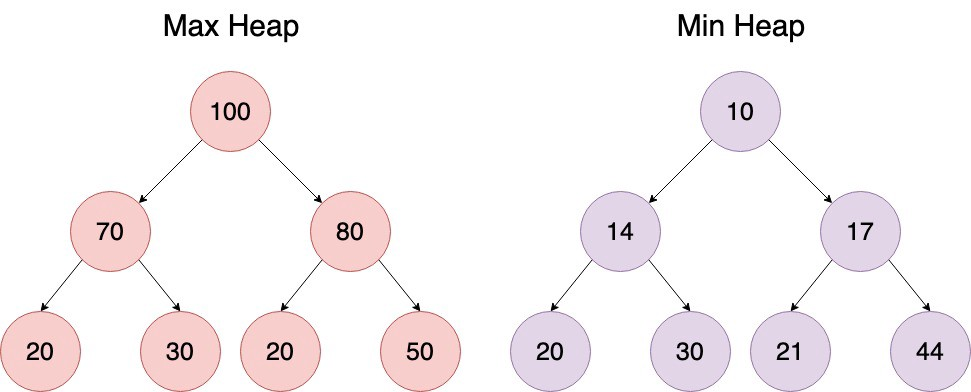
\includegraphics[width=1\linewidth]{1*EU964HO0LZyypp7_MLkY8A}
		\label{fig:1eu964ho0lzyypp7mlky8a}
	\end{figure}
	\alert{Heaps are not sorted}
\end{frame}

\begin{frame}
	\frametitle	{Heap as a Tree} 
	\begin{itemize}
		\item \textcolor{blue} {root of tree:} first element in the array, corresponding to i = 1 \item \textcolor{blue}{parent(i) =i/2:} returns index of node's parent
		\item \textcolor{blue}{left(i)=2i:} returns index of node's left child
		\item \textcolor{blue}{right(i)=2i+1:} returns index of node's right child
	\end{itemize}
\end{frame}

\begin{frame}
	\frametitle	{Heap as a Tree} 
    \begin{figure}
    	\centering
    	\includegraphics[width=1.09\linewidth]{"Screenshot 2020-12-23 at 8.48.18 PM"}
    	\label{fig:screenshot-2020-12-23-at-8}
    \end{figure}    
\end{frame}

\begin{frame}
	\frametitle	{Heap Operation} 
    \begin{itemize}
    		\item \textcolor{blue}{build\_max\_heap :} produce a max-heap from an unordered array
    	 	\item \textcolor{blue}{max\_heapify :} correct a \alert{single} violation of the heap property in a subtree at its root
    \end{itemize}
\end{frame}

\begin{frame}
	\frametitle	{Max\_Heapify} 
	\begin{itemize}
		\item Assume that the trees rooted at left(i) and right(i) are max-heaps
		\item If element A[i] violates the max-heap property, correct violation by “trickling” element A[i] down the tree, making the subtree rooted at index i a max-heapt
	\end{itemize}
\end{frame}

\begin{frame}
	\frametitle	{Max\_Heapify Example} 
	\begin{figure}
		\centering
		\includegraphics[width=1\linewidth]{"Screenshot 2020-12-23 at 9.03.40 PM"}
		\label{fig:screenshot-2020-12-23-at-9}
	\end{figure}
	
\end{frame}

\begin{frame}
	\frametitle	{Max\_Heapify Example} 
	\begin{figure}
		\centering
		\includegraphics[width=1\linewidth]{"Screenshot 2020-12-23 at 9.03.53 PM"}
		\label{fig:screenshot-2020-12-23-at-9}
	\end{figure}	
\end{frame}

\begin{frame}
	\frametitle	{Max\_Heapify Example} 
	\begin{figure}
		\centering
		\includegraphics[width=1\linewidth]{"Screenshot 2020-12-23 at 9.04.07 PM"}
		\label{fig:screenshot-2020-12-23-at-9}
	\end{figure}	
\end{frame}

\begin{frame}
	\frametitle	{Max\_Heapify Running time???} 
	\pause O(log n)
\end{frame}

\begin{frame}
	\frametitle	{build\_max\_heap(A)} 
	
	Converts A[1...n] to a max heap\\
	Build\_Max\_Heap(A):\\ for i=n/2 downto 1\\
	do Max\_Heapify(A, i)\\
	\pause \alert{Why start at n/2?}\\
	\pause \textcolor{blue}{Because elements A[n/2 + 1 ... n] are all leaves of the tree 2i > n, for i > n/2 + 1}
\end{frame}

\begin{frame}
	\frametitle	{build\_max\_heap(A) Demo} 
	\begin{figure}
		\centering
		\includegraphics[width=1\linewidth]{"Screenshot 2020-12-23 at 9.29.55 PM"}
		\label{fig:screenshot-2020-12-23-at-9}
	\end{figure}
	
\end{frame}

\begin{frame}
	\frametitle	{build\_max\_heap(A) Demo} 
	\begin{figure}
		\centering
		\includegraphics[width=1\linewidth]{"Screenshot 2020-12-23 at 9.30.04 PM"}
		\label{fig:screenshot-2020-12-23-at-9}
	\end{figure}
	
\end{frame}

\begin{frame}
	\frametitle	{build\_max\_heap(A) Demo} 
	\begin{figure}
		\centering
		\includegraphics[width=1\linewidth]{"Screenshot 2020-12-23 at 9.30.18 PM"}
		\label{fig:screenshot-2020-12-23-at-9}
	\end{figure}
	
\end{frame}

\begin{frame}
	\frametitle	{build\_max\_heap(A) Demo} 
	\begin{figure}
		\centering
		\includegraphics[width=1\linewidth]{"Screenshot 2020-12-23 at 9.30.27 PM"}
		\label{fig:screenshot-2020-12-23-at-9}
	\end{figure}
	
\end{frame}

\begin{frame}
	\frametitle	{build\_max\_heap(A) Demo} 
	\begin{figure}
		\centering
		\includegraphics[width=1\linewidth]{"Screenshot 2020-12-23 at 9.30.40 PM"}
		\label{fig:screenshot-2020-12-23-at-9}
	\end{figure}
	
\end{frame}

\begin{frame}
	\frametitle	{build\_max\_heap(A) Running time???} 
	\pause O(n log n)
\end{frame}


\begin{frame}
	\frametitle	{HeapSort} 
	Sorting Strategy:
    \begin{enumerate}
    	\item Build Max Heap from unordered array;
    	\item  Find maximum element A[1];
    	\item Swap elements A[n] and A[1]: now max element is at the end of the array!
    	\item Discard node n from heap(by decrementing heap-size variable)
    	\item New root may violate max heap property, but its children are max heaps. Run max\_heapify to fix this.
    	\item Go to Step 2 unless heap is empty.
    \end{enumerate}
\end{frame}

\begin{frame}
	\frametitle	{HeapSort Example} 
	\begin{figure}
		\centering
		\includegraphics[width=1\linewidth]{"Screenshot 2020-12-23 at 9.42.04 PM"}
		\label{fig:screenshot-2020-12-23-at-9}
	\end{figure}
	
\end{frame}

\begin{frame}
	\frametitle	{HeapSort Example} 
	\begin{figure}
		\centering
		\includegraphics[width=1\linewidth]{"Screenshot 2020-12-23 at 9.42.11 PM"}
		\label{fig:screenshot-2020-12-23-at-9}
	\end{figure}
	
\end{frame}
\begin{frame}
	\frametitle	{HeapSort Example} 
	\begin{figure}
		\centering
		\includegraphics[width=1\linewidth]{"Screenshot 2020-12-23 at 9.42.18 PM"}
		\label{fig:screenshot-2020-12-23-at-9}
	\end{figure}
	
\end{frame}
\begin{frame}
	\frametitle	{HeapSort Example} 
	\begin{figure}
		\centering
		\includegraphics[width=1\linewidth]{"Screenshot 2020-12-23 at 9.42.25 PM"}
		\label{fig:screenshot-2020-12-23-at-9}
	\end{figure}
	
\end{frame}
\begin{frame}
	\frametitle	{HeapSort Example} 
	\begin{figure}
		\centering
		\includegraphics[width=1\linewidth]{"Screenshot 2020-12-23 at 9.42.34 PM"}
		\label{fig:screenshot-2020-12-23-at-9}
	\end{figure}
	
\end{frame}
\begin{frame}
	\frametitle	{HeapSort Example} 
	\begin{figure}
		\centering
		\includegraphics[width=1\linewidth]{"Screenshot 2020-12-23 at 9.42.43 PM"}
		\label{fig:screenshot-2020-12-23-at-9}
	\end{figure}
\end{frame}

\begin{frame}
	\alert{THANK YOU FOR YOUR TIME. BEST OF LUCK IN YOUR EXAM}
\end{frame}
\end{document}